\chapter{Risultati sperimentali}\label{ch:risultati}
\section{Validation principale e selezione}
La verifica degli aggregati identifica 36 run uniche e cinque famiglie complete a ciascuna profondità. Le tabelle seguenti usano i campi con cutoff esplicito. La Tabella~\ref{tab:validation} riporta le cinque configurazioni selezionate nello scenario $N=100$. TN indica Track Novelty, AN Artist Novelty; NDCG, TN, AN e ILD sono a $K=10$, mentre Reward riguarda la Top-1.

\begin{table}[htbp]\centering\footnotesize
\begin{tabular}{lrrrrrrr}
\toprule
Policy & NDCG & Prec. & Recall & Reward & TN & AN & ILD \\
\midrule
Random & 0,066118 & 0,066361 & 0,013014 & 0,097295 & 0,879464 & 0,467697 & 0,993623 \\
Global Popularity & 0,041145 & 0,185827 & 0,003604 & 0,308597 & 0,668625 & 0,238711 & 0,000000 \\
Personalized Greedy & 0,276427 & 0,394560 & 0,052080 & 1,060560 & 0,448995 & 0,000000 & 0,756039 \\
$\varepsilon$-Greedy & 0,265987 & 0,378354 & 0,049943 & 1,012495 & 0,470583 & 0,023278 & 0,767605 \\
LinUCB & 0,285640 & 0,362577 & 0,054551 & 1,003704 & 0,551388 & 0,043548 & 0,830548 \\
\bottomrule
\end{tabular}

\caption{Validation a $N=100$: $\varepsilon=0{,}05$, $\alpha=2$. Metriche a @10, reward Top-1.}\label{tab:validation}
\end{table}

LinUCB raggiunge NDCG@10 0,285640, contro 0,276427 di Personalized Greedy e 0,265987 di $\varepsilon$-Greedy. La reward media più alta fra queste tre configurazioni è invece quella di Greedy, pari a 1,060560. La scelta di LinUCB nella propria famiglia segue la metrica primaria, senza sostituirla con la reward dopo aver visto il risultato.

Lo sweep $\alpha$ non è strettamente monotono: a $N=100$ il valore 0,25 è leggermente inferiore a 0,1; da 0,5 a 2 NDCG cresce moderatamente. La differenza fra le migliori impostazioni è piccola rispetto alla separazione da Random e Popularity. Il valore $\alpha=0$ produce 0,270426: la componente lineare e la sua traiettoria di aggiornamento costituiscono già una policy distinta da Greedy.

Per $\varepsilon$-Greedy l'aumento da 0,05 a 0,10 e 0,20 riduce NDCG@10 da 0,265987 a 0,254587 e 0,234917, e la reward da 1,012495 a 0,960985 e 0,870854. In questo ambiente una maggiore frazione di ranking casuali penalizza l'allineamento agli ascolti futuri. Non dimostra che l'esplorazione sia inutile in generale: Random offre la massima varietà ma non impiega preferenze, e il dataset non registra eventuali nuovi ascolti causati dall'esposizione.

\figura{sweeps.pdf}{1}{Sweep di validation. La selezione usa esclusivamente la curva $N=100$; le altre due descrivono la sensibilità.}{fig:sweeps}

\section{Sensibilità alla profondità}
La Tabella~\ref{tab:sensitivity} mantiene gli iperparametri congelati anche per $N=50$ e $N=200$, così il confronto mostra l'effetto dell'ambiente candidato. Non va interpretata come una nuova ottimizzazione degli iperparametri per ciascun $N$.
\begin{table}[htbp]\centering\small
\begin{tabular}{lrrrrr}
\toprule
N & Policy & NDCG@10 & Reward & AN@10 & ILD@10 \\
\midrule
50 & Random & 0,065606 & 0,095330 & 0,470296 & 0,993194 \\
50 & Global Popularity & 0,052096 & 0,308597 & 0,256800 & 0,125482 \\
50 & Personalized Greedy & 0,268507 & 0,975219 & 0,000000 & 0,790844 \\
50 & $\varepsilon$-Greedy & 0,258463 & 0,931208 & 0,023026 & 0,800752 \\
50 & LinUCB & 0,263452 & 0,928883 & 0,059524 & 0,852294 \\
100 & Random & 0,066118 & 0,097295 & 0,467697 & 0,993623 \\
100 & Global Popularity & 0,041145 & 0,308597 & 0,238711 & 0,000000 \\
100 & Personalized Greedy & 0,276427 & 1,060560 & 0,000000 & 0,756039 \\
100 & $\varepsilon$-Greedy & 0,265987 & 1,012495 & 0,023278 & 0,767605 \\
100 & LinUCB & 0,285640 & 1,003704 & 0,043548 & 0,830548 \\
200 & Random & 0,063062 & 0,091953 & 0,478737 & 0,995699 \\
200 & Global Popularity & 0,041145 & 0,308597 & 0,238711 & 0,000000 \\
200 & Personalized Greedy & 0,273409 & 1,132060 & 0,000000 & 0,703238 \\
200 & $\varepsilon$-Greedy & 0,262647 & 1,081188 & 0,024616 & 0,718212 \\
200 & LinUCB & 0,293715 & 1,097895 & 0,025820 & 0,785190 \\
\bottomrule
\end{tabular}

\caption{Sensibilità della validation con $\alpha=2$ ed $\varepsilon=0{,}05$ mantenuti fissi.}\label{tab:sensitivity}
\end{table}

L'effetto di $N$ non è un semplice aumento della stessa lista: nuove tracce modificano la scelta Top-1, la composizione delle Top-K e, per LinUCB, la sequenza delle reward e degli aggiornamenti. Cambia inoltre il campione dei contesti su cui è stimato lo scaler. Una differenza fra due profondità comprende quindi tutti questi effetti. Anche i denominatori della coverage seguono il catalogo effettivamente esposto.

Il massimo numerico dell'intera griglia può trovarsi fuori dallo scenario principale. Ad esempio, a $N=200$ LinUCB con $\alpha=1$ raggiunge NDCG@10 circa 0,293811, superiore al valore con $\alpha=2$ della stessa profondità. Questa osservazione resta sensibilità: non cambia la selezione nello scenario $N=100$ definito prima della validation. La griglia completa è riportata nell'Appendice~\ref{app:repro}.

\section{Test held-out e confronto con la validation}
Le cinque policy congelate sono tutte presenti una volta nell'aggregato del test. Nessuna configurazione è scelta sulla base della tabella held-out. Il ranking per NDCG@10 cambia nelle prime due posizioni: Personalized Greedy supera numericamente LinUCB di circa 0,001055. L'analisi appaiata del Capitolo~\ref{ch:stat} serve a quantificare l'incertezza di questo scarto.

\begin{table}[htbp]\centering\footnotesize
\begin{tabular}{lrrrrrrr}
\toprule
Policy & NDCG & Prec. & Recall & Reward & TN & AN & ILD \\
\midrule
Random & 0,058348 & 0,058273 & 0,012488 & 0,083866 & 0,881662 & 0,465040 & 0,993400 \\
Global Popularity & 0,036927 & 0,164711 & 0,003878 & 0,266868 & 0,650198 & 0,220333 & 0,000000 \\
Personalized Greedy & 0,258795 & 0,364422 & 0,053806 & 0,973338 & 0,448135 & 0,000000 & 0,752957 \\
$\varepsilon$-Greedy & 0,248893 & 0,349606 & 0,051404 & 0,929997 & 0,469995 & 0,023193 & 0,764725 \\
LinUCB & 0,257741 & 0,320681 & 0,054112 & 0,913353 & 0,556484 & 0,101535 & 0,832490 \\
\bottomrule
\end{tabular}

\caption{Risultati held-out a $N=100$. Le metriche di lista sono a @10 e la reward è Top-1. L'ordine delle righe identifica le famiglie, non una nuova selezione.}\label{tab:test}
\end{table}

Greedy mantiene la reward media più alta, 0,973338; LinUCB ottiene 0,913353 ed $\varepsilon$-Greedy 0,929997. LinUCB propone però più item mai ascoltati: TN@10 è 0,556484, contro 0,448135 di Greedy. La AN@10 passa da zero a 0,101535 e ILD@10 da 0,752957 a 0,832490. L'esplorazione di nuove identità è quindi osservabile nei ranking, pur non trasformandosi automaticamente in reward maggiore.

La divergenza, già presente in validation, motiva entrambe le misure: ordinare artisti pertinenti non equivale a scegliere la Top-1 con più riascolti.

\figura{validation_test.pdf}{1}{Confronto descrittivo a $N=100$ fra validation e test, con gli stessi parametri selezionati. I pannelli hanno scale diverse e misurano obiettivi distinti.}{fig:valtest}

\begin{table}[htbp]\centering\small
\begin{tabular}{lrrrrr}
\toprule
Policy & Val. & Test & $\Delta$ NDCG & $\Delta$ rel. & $\Delta$ Reward \\
\midrule
Random & 0,066118 & 0,058348 & -0,007770 & -11,75\% & -0,013430 \\
Global Popularity & 0,041145 & 0,036927 & -0,004218 & -10,25\% & -0,041730 \\
Personalized Greedy & 0,276427 & 0,258795 & -0,017632 & -6,38\% & -0,087223 \\
$\varepsilon$-Greedy & 0,265987 & 0,248893 & -0,017094 & -6,43\% & -0,082498 \\
LinUCB & 0,285640 & 0,257741 & -0,027899 & -9,77\% & -0,090351 \\
\bottomrule
\end{tabular}

\caption{Variazioni test meno validation. La variazione relativa riguarda NDCG@10; la reward è confrontata in differenza assoluta.}\label{tab:valtest}
\end{table}

Tutte le famiglie ottengono un NDCG@10 inferiore nel test. Ciò è compatibile con un cambiamento temporale di interessi o catalogo, ma non ne identifica da solo la causa. Validation e test hanno durate e opportunità diverse; il valore medio della reward è inoltre sensibile all'intensità degli ascolti futuri. Non è corretto interpretare la variazione come un peggioramento causato dall'algoritmo.

\par\noindent\begin{minipage}{\linewidth}
Global Popularity è un caso istruttivo: TN@10 è 0,650198, ma ILD@10 è zero e Artist Coverage@10 circa 0,000319. Una traccia può essere nuova anche appartenendo all'artista ripetuto in tutta la lista. L'ordinamento per artista permette a più sue tracce di occupare le prime posizioni. La deduplicazione artist-level per NDCG evita di contare più volte quella stessa pertinenza, ma non corregge la composizione del ranking prodotto.
\end{minipage}\par

\begin{table}[htbp]\centering\scriptsize
\begin{tabular}{lrrrrrr}
\toprule
Policy & $C_I@5$ & $C_G@5$ & $C_I@10$ & $C_G@10$ & $C_I@20$ & $C_G@20$ \\
\midrule
Random & 0,842371 & 0,888960 & 0,911745 & 0,940970 & 0,954116 & 0,969049 \\
Global Popularity & 0,002195 & 0,000319 & 0,004391 & 0,000319 & 0,009879 & 0,001276 \\
Personalized Greedy & 0,195390 & 0,199426 & 0,283425 & 0,285578 & 0,410757 & 0,415444 \\
$\varepsilon$-Greedy & 0,428321 & 0,474474 & 0,545774 & 0,596362 & 0,681668 & 0,730057 \\
LinUCB & 0,292426 & 0,314295 & 0,385071 & 0,416401 & 0,508233 & 0,548819 \\
\bottomrule
\end{tabular}

\caption{Coverage held-out distinta per cutoff. $C_I$ è catalog coverage e $C_G$ artist coverage; gli alias senza suffisso del CSV corrispondono alle ultime due colonne.}\label{tab:coverage}
\end{table}

Random esplora gran parte del catalogo ma ottiene NDCG basso. $\varepsilon$-Greedy copre più catalogo di LinUCB grazie alle permutazioni casuali, mentre LinUCB migliora novelty e ILD medie rispetto a $\varepsilon$-Greedy. Coverage e varietà della singola lista non sono intercambiabili: una policy può distribuire nel tempo poche raccomandazioni casuali su molti item, restando per la maggioranza delle decisioni concentrata sui contenuti noti.

\section{Cutoff ed esempi qualitativi}
La Tabella~\ref{tab:cutoffs} rende espliciti anche i cutoff 5 e 20. Allungare la lista cambia sia il numero di tracce sia quello di artisti distinti disponibili alla metrica. Le metriche a cutoff diversi non sono repliche indipendenti, perché usano prefissi dello stesso ranking.
\begin{table}[htbp]\centering\scriptsize
\begin{tabular}{lrrrrrrr}
\toprule
Policy & K & NDCG & Prec. & Recall & TN & AN & ILD \\
\midrule
Random & 5 & 0,059115 & 0,059437 & 0,006425 & 0,881678 & 0,462700 & 0,993376 \\
Random & 20 & 0,057709 & 0,056549 & 0,023137 & 0,881825 & 0,469460 & 0,993287 \\
Global Popularity & 5 & 0,056281 & 0,164711 & 0,003878 & 0,642070 & 0,220333 & 0,000000 \\
Global Popularity & 20 & 0,041048 & 0,136021 & 0,008740 & 0,669677 & 0,238681 & 0,338792 \\
Personalized Greedy & 5 & 0,299744 & 0,403090 & 0,036630 & 0,428003 & 0,000000 & 0,703799 \\
Personalized Greedy & 20 & 0,226655 & 0,312121 & 0,076603 & 0,484342 & 0,000000 & 0,802236 \\
$\varepsilon$-Greedy & 5 & 0,288001 & 0,386336 & 0,034984 & 0,450852 & 0,022893 & 0,718243 \\
$\varepsilon$-Greedy & 20 & 0,218264 & 0,299679 & 0,073656 & 0,504320 & 0,023286 & 0,811658 \\
LinUCB & 5 & 0,299467 & 0,367270 & 0,038040 & 0,542255 & 0,070830 & 0,797706 \\
LinUCB & 20 & 0,221357 & 0,262718 & 0,075783 & 0,583223 & 0,157702 & 0,874082 \\
\bottomrule
\end{tabular}

\caption{Metriche held-out a @5 e @20. TN, AN e ILD conservano le definizioni del Capitolo~\ref{ch:metodo}.}\label{tab:cutoffs}
\end{table}

Gli esempi U01--U05 sono quelli già selezionati e verificati nel notebook ufficiale. La cache contiene 150 raccomandazioni Top-10, corrispondenti a 98 item distinti con metadati recuperati. Non è un campione casuale rappresentativo: serve a mostrare differenze di composizione e non a stimare la frequenza dei casi favorevoli. Qui si riportano due episodi che mostrano esiti diversi; non è stata effettuata una nuova selezione sull'held-out.

\begin{table}[htbp]\centering\small
\begin{tabular}{lp{2.6cm}p{4.3cm}rr}
\toprule
Policy & Artista Top-1 & Titolo Top-1 & Reward & Nuovi \\
\midrule
Personalized Greedy & Johnny Cash & Hurt & 3,496508 & 0 \\
LinUCB & Fractal Pattern & Ad Infinitum & 0,000000 & 0 \\
$\varepsilon$-Greedy & Tool & Bottom (Feat. Henry Rollins) & 2,564949 & 7 \\
\bottomrule
\end{tabular}

\caption{U01, 01/03/2009 alle 11:44:06. La colonna Nuovi conta gli artisti distinti nuovi nelle Top-10; la reward riguarda solo la Top-1.}\label{tab:u01}
\end{table}

In U01 Greedy propone \emph{Hurt} di Johnny Cash, con reward $\ln(33)=3{,}496508$, mentre LinUCB sceglie \emph{Ad Infinitum} di Fractal Pattern, senza ascolti futuri dell'artista nella finestra. Entrambe le liste hanno zero artisti nuovi: una raccomandazione diversa non è necessariamente una nuova identità artista. $\varepsilon$-Greedy propone Tool come Top-1 e include sette artisti nuovi nelle Top-10. Il caso non favorisce LinUCB ed evidenzia che il bonus non garantisce pertinenza locale.

\begin{table}[htbp]\centering\small
\begin{tabular}{lp{2.6cm}p{4.3cm}rr}
\toprule
Policy & Artista Top-1 & Titolo Top-1 & Reward & Nuovi \\
\midrule
Personalized Greedy & Kings Of Leon & Charmer & 0,693147 & 0 \\
LinUCB & Roy Hargrove & Frosty The Snowman & 0,000000 & 10 \\
$\varepsilon$-Greedy & Kings Of Leon & Charmer & 0,693147 & 0 \\
\bottomrule
\end{tabular}

\caption{U04, 09/04/2009 alle 15:08:15. Esempio di lista LinUCB composta da dieci artisti nuovi senza riscontro Top-1 nella reward proxy.}\label{tab:u04}
\end{table}

In U04 LinUCB seleziona Roy Hargrove e presenta dieci artisti nuovi, ma il proxy Top-1 è zero; Greedy ed $\varepsilon$-Greedy coincidono su Kings of Leon e ottengono $\ln(2)$. Si tratta di un compromesso reale fra apertura della lista e riscontro storico futuro. La cache conserva flag esatti di \emph{artist novelty}; non conserva la storia item completa per ricostruire la track novelty di questi esempi. La TN aggregata ufficiale rimane valida e viene analizzata separatamente. Nessuno dei riscontri futuri dimostra che la raccomandazione abbia causato un ascolto.

\begin{figure}[p]\centering
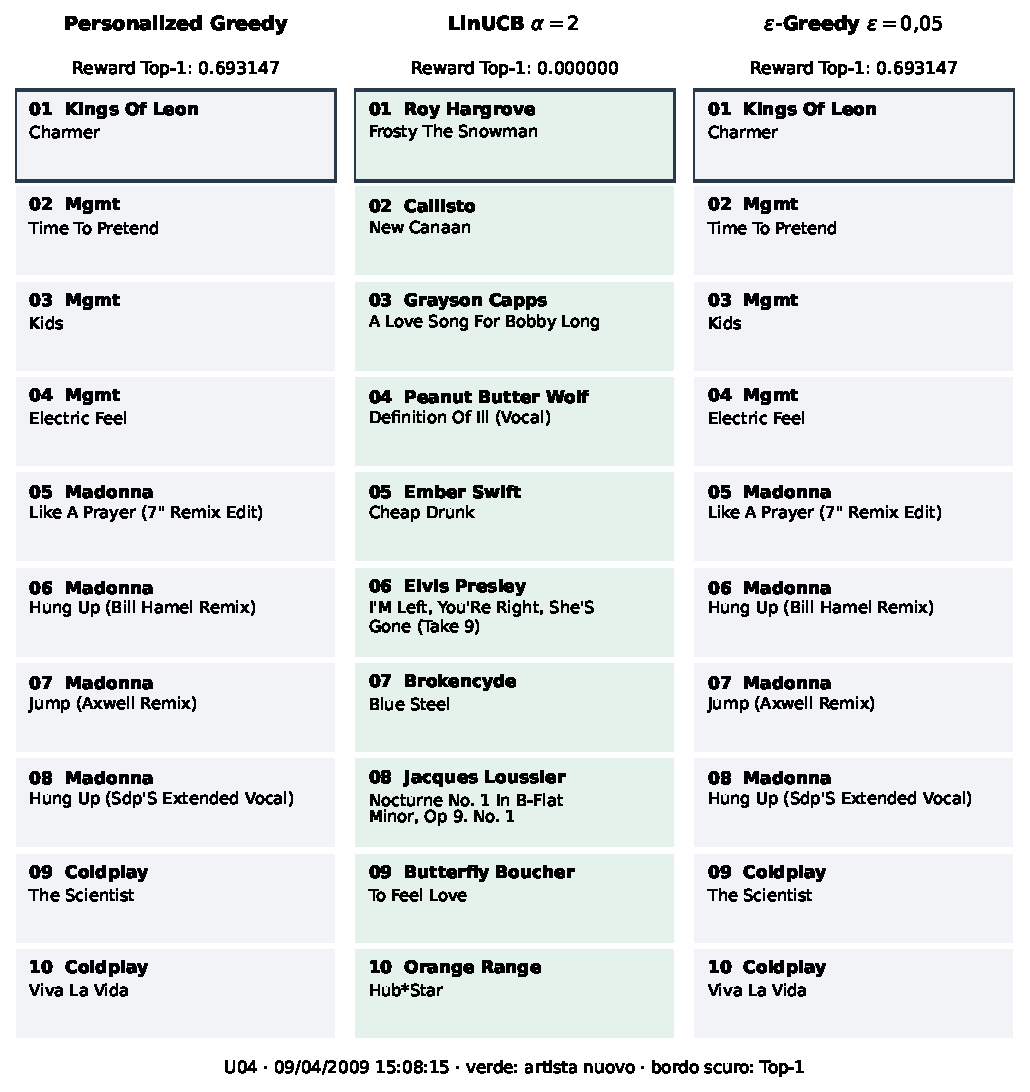
\includegraphics[width=\linewidth]{qualitative_U04.pdf}
\caption{Top-10 reali per U04, stesso utente e istante della Tabella~\ref{tab:u04}. Il verde contrassegna un artista mai ascoltato prima del decision point; il bordo scuro evidenzia la Top-1. Greedy ed $\varepsilon$-Greedy coincidono, mentre LinUCB cambia tutti gli artisti. Titoli, ordine, flag e reward sono letti dalla cache verificata, senza scansioni o nuove decisioni. Un artista nuovo non implica un successivo ascolto.}\label{fig:qualitative}
\end{figure}
